\section{Introduction}\label{sec:intro}
UNICEF and Solve for Good have partnered together to analyze various aspects of changes in air pollution — especially related to COVID-19 and with the long-term goal to build a platform for air pollution monitoring with a strong emphasis on UNICEF’s operations, with focus on
\begin{itemize}
    \item Developing a model to measure children’s exposure to air pollutant PM2.5, which exceeds the WHO Standard in the present COVID Scenario.
    \item Understanding the air quality level around the globe with the target of attaining a fine-grained estimation from the combination of Ground value measurement from openly available ground sensor measurements and Remote Sensing
    \item Enabling Citizen Scientists to delve deeper and get involved in Air Quality Measurement globally.
\end{itemize} 
%
Specifically, we aim to (a) model the impact of COVID19 lockdowns on air quality and (b) test whether this has led to an improvement in children’s health. Following the footsteps of existing works like \citet{Borneman,Mahato}, we hypothesize to find evidence of the positive effects of air quality resulting from the large-scale modal shift to low emissions vehicles post lockdown develop an exploratory visualization platform for local program managers. The platform will provide functions to manage, analyze, and visualize changes in air pollution data at different locations preferably, in countries and cities where UNICEF operates with interests in air pollution monitoring for children’s health.

Globally, 93\% of children live in environments where air pollution levels exceed WHO guidelines. There is a strong link between human health and exposure to high levels of air pollution. Long-term exposure to fine particulate matter with a diameter less than 2.5$\mu$m (PM2.5) are estimated to cause ~8 million excess deaths annually. Simultaneously, nitrogen dioxide (NO$_2$) results in 4 million new pediatric asthma cases annually \cite{Venter}. The impact of air pollution is felt more acutely by the young, with one in every four deaths of children under 5 years is directly or indirectly related to environmental risks \cite{who}.

However, the child population’s distribution does not correspond well to the global distribution of air quality sensors. Illustrating these distributions are panel (a) of Figure~\ref{fig:maps} showing the locations of air quality sensors and panel (b) the global concentration of child populations. Therefore using only the locations of ground-source air quality sensors to infer the effects of exposure to high levels of air pollution on global child populations is difficult, particularly in high populous locations such as Western Africa and the Great Rift Valley.

\begin{figure*}
    \centering
    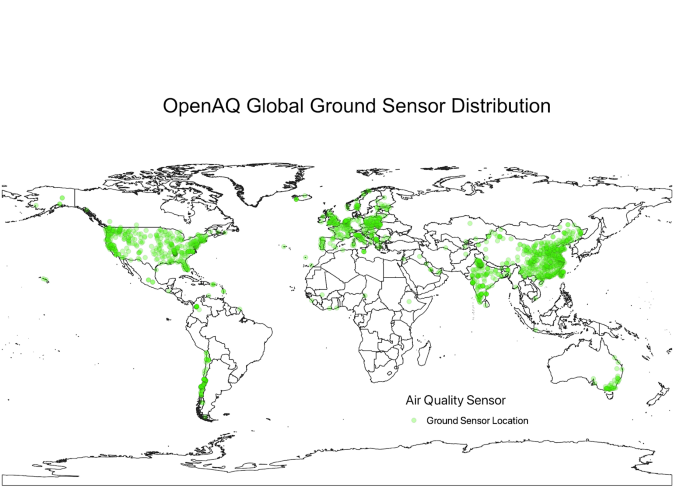
\includegraphics[width=.49\textwidth]{sensormap.png}
    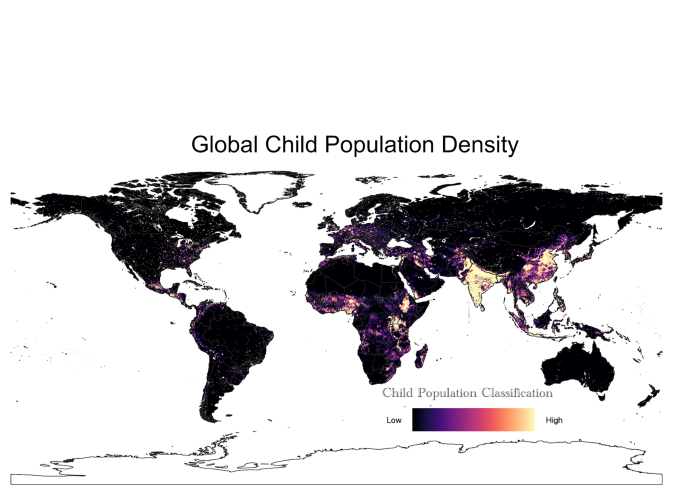
\includegraphics[width=.49\textwidth]{childmap.png}
    \caption{Global distribution of (a) air quality sensors, and (b) Child Population, data source: Silent Suffocation in Africa, UNICEF-2019.}
    \label{fig:maps}
\end{figure*}

During the Covid-19 lockdowns, fossil fuel consumption has decreased due to lower mobility levels in general, as well as a shift to low-emission modes of transport (such as walking and cycling). This prevents previous models that measure the global distribution of air pollution inaccurate, as they are unable to represent the current changes in air pollution levels due to COVID19 lockdown events \cite{stateof}.

The decreased concentration of harmful emissions resulting from this has the potential to significantly improve cardiovascular health for children, who are more vulnerable to the impact of air pollution \cite{Rees}. At UNICEF and Solve for Good, we wanted to question the children’s health to the global air quality emissions data UNICEF collected during the lockdown to identify if there is a significant improvement in child health with a mass transition to low carbon energy sources for industry and vehicles.
We take a 3 step approach to our analysis.

\begin{enumerate}
    \item We develop a large-scale model aimed at providing air quality predictions across geographic regions using widely available data sources,
    \item Develop a geospatial visualization platform for the exploration of results,
    \item Fine-tune results of the large-scale model using location-specific heterogeneous data sources for more accurate local-level predictions, and correlate results with child health indicators.
\end{enumerate}

%We focus on the first two steps in this article series. The first article discusses the importance of air quality monitoring, the available data sources, data setup, and some exploratory results in the current context. In the second article, we shall discuss the details and results pertaining to the global level model. The third article will be aimed at visualization and discussion of results, as well as pointers towards future work on local models and incorporating child health data.